
\section{Stochastic Campaign}\label{results:stochastic}

The generation of exchanges is designed as a stochastic process. Each reactor is
assigned a target enrichment per consumable commodity in a given range, and each
facility is assigned a location value. Enrichment stochasticity results in
perturbed constraint matrix coefficients, and location stochasticity results in
perturbed objective coefficient if $f_{\text{loc}}$ is set to include
location-based preference.

In \secref{results:scale}, a single exchange instance was investigated for each
solver as problem size scale was investigated. While clear patterns were
inferred as a result of the study, stochastic effects were left
unexplored. Accordingly, a second study was undertaken in order to examine how
sensitive both solution values and execution time are to randomness in instance
generation.

For this study, instances are generated for a single parameter vector. It is
best to compare converged \cbc solutions for confidence in the resulting
objective value and in order to run all desired instances in a reasonable amount
of time. Accordingly, the total reactor population was set at 65 based on the
scaling study results. Specifically, this is approximately the largest reactor
population for which all configurations of parameters converged (see Figure
\ref{fig:base_front_n_rxtr_time_fc0_cbc}). For each combination of fundamental
parameters, 1000 instances were generated and executed by each solver for both
front and back-end exchanges.

In both sections, cumulative observations are presented. Figures are presented
in two panes for a given fuel cycle, with low-fidelity reactor instances on the
left and high-fidelity reactor instances on the right. In each pane, the results
for all three location fidelity parameters are shown.

\subsection{Front-End Exchanges}

\subsubsection{Fundamental Parameter Variation}

The Greedy Solver and \clp both proved to have relatively stable solution
times. The timing results are similar across fuel cycles. Accordingly, MOX fuel
cycle results are shown for the Greedy Solver in Figure
\ref{fig:1k_avg_front_time_fc1_greedy}, and \clp results are shown in Figure
\ref{fig:1k_avg_front_time_fc1_clp}. Apart from solution time stability, the
primary observation for both the \clp and Greedy solvers is related to location
fidelity effects. Although there is a ranking in average solution time by
location parameter \textit{for a given collection of fundamental parameters},
that ranking changes for each collection of parameters, as can be seen in the
presented figures.

\begin{figure}[h!]
  \begin{center}
    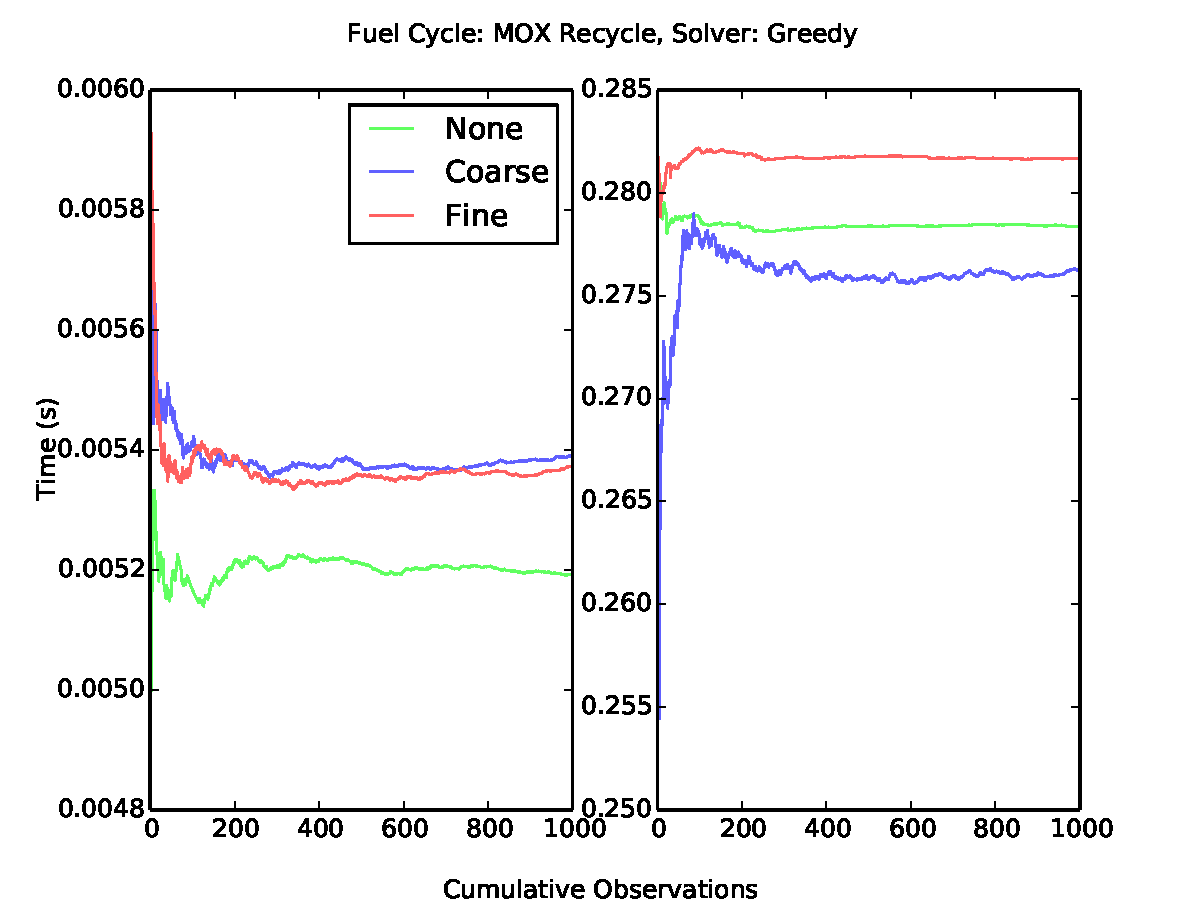
\includegraphics[width=.7\textwidth]{1k_avg_front_time_fc1_greedy.pdf}
    \caption{
      \label{fig:1k_avg_front_time_fc1_greedy}
      Cumulative average solution time of the Greedy solver for the front-end
      MOX fuel cycle. Low-fidelity reactor instances comprise the left pane, and
      high-fidelity reactor instances comprise the right pane. Each colored line
      represents a different objective coefficient location fidelity.}
  \end{center}
\end{figure}

\begin{figure}[h!]
  \begin{center}
    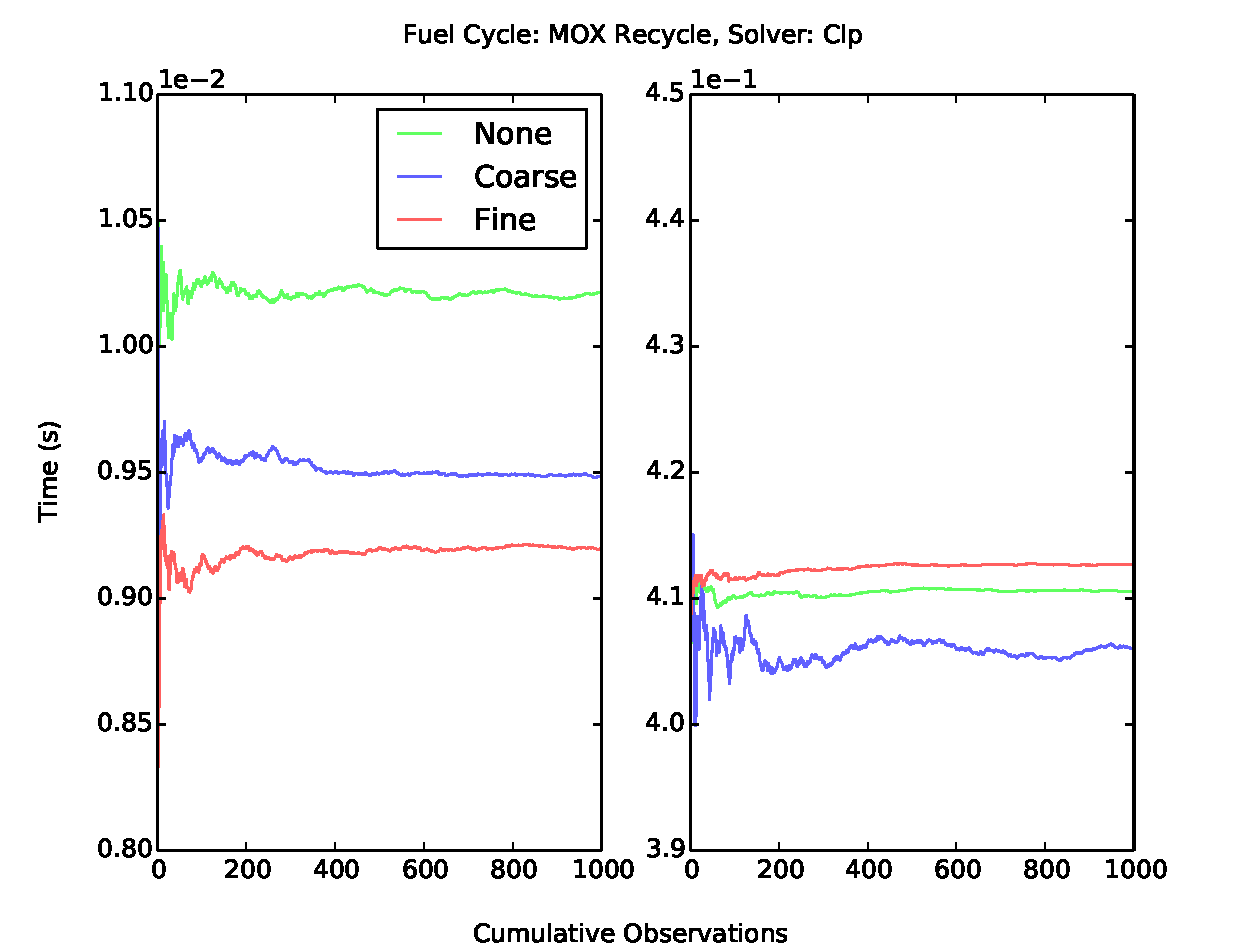
\includegraphics[width=.7\textwidth]{1k_avg_front_time_fc1_clp.pdf}
    \caption{
      \label{fig:1k_avg_front_time_fc1_clp}
      Cumulative average solution time of the \clp solver for the front-end MOX fuel
      cycle.}
  \end{center}
\end{figure}

The \cbc solver showed much less stability in solution times. Further, behavior
was found to be different for each fuel
cycle. \Cref{fig:1k_avg_front_time_fc0_cbc,fig:1k_avg_front_time_fc1_cbc,fig:1k_avg_front_time_fc2_cbc}
show the timing results for the OT, MOX, and ThOX fuel cycles,
respectively. 

\begin{figure}[h!]
  \begin{center}
    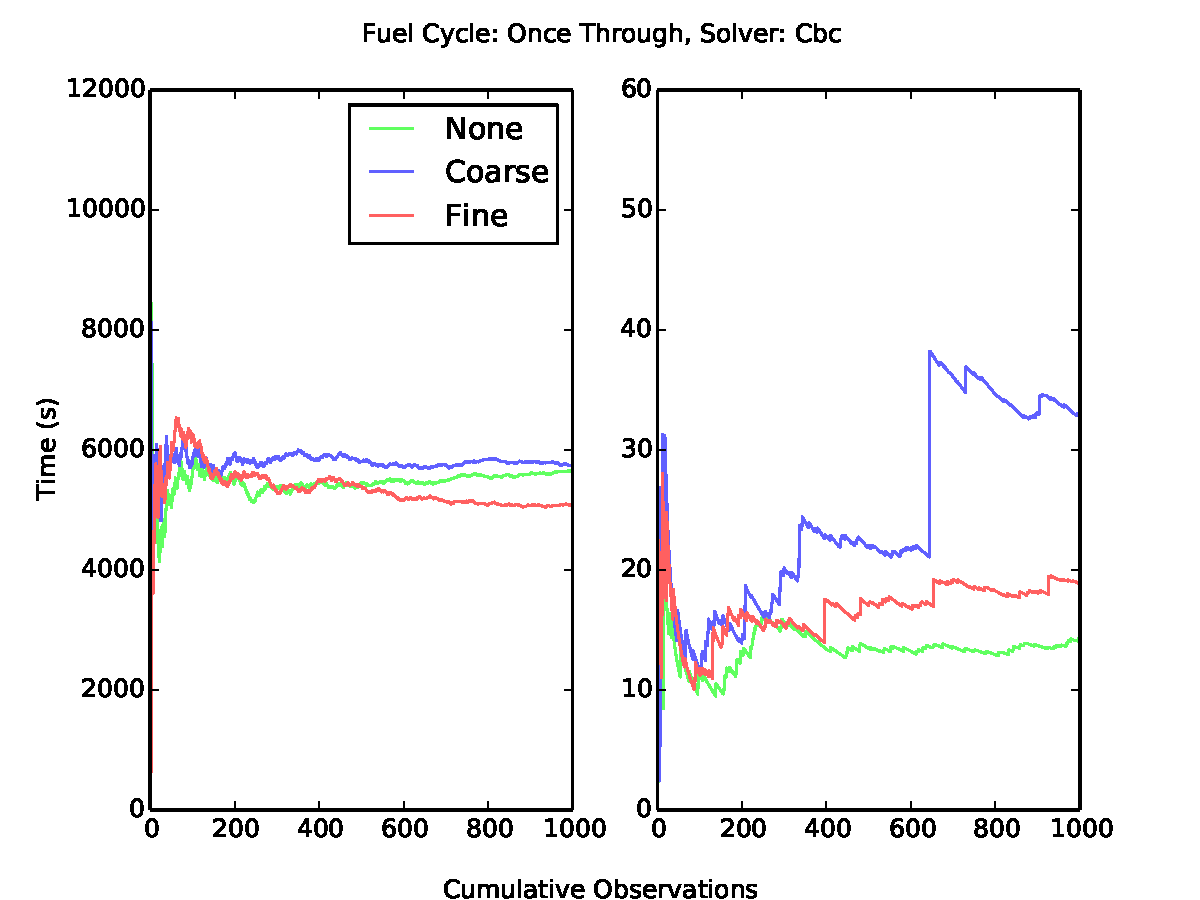
\includegraphics[width=.7\textwidth]{1k_avg_front_time_fc0_cbc.pdf}
    \caption{
      \label{fig:1k_avg_front_time_fc0_cbc}
      Cumulative average solution time of the \cbc solver for the front-end
      once-through fuel cycle.}
  \end{center}
\end{figure}

\begin{figure}[h!]
  \begin{center}
    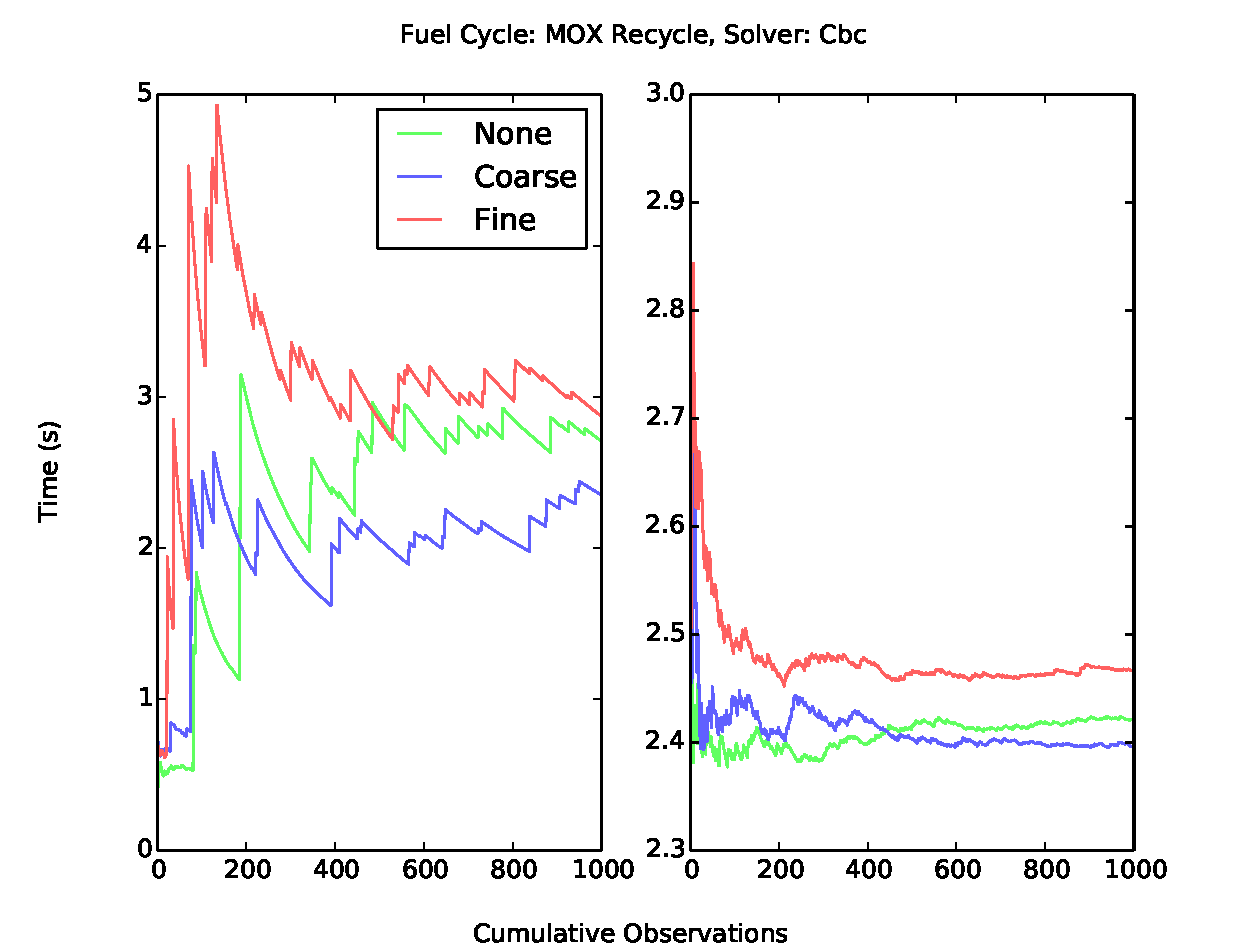
\includegraphics[width=.7\textwidth]{1k_avg_front_time_fc1_cbc.pdf}
    \caption{
      \label{fig:1k_avg_front_time_fc1_cbc}
      Cumulative average solution time of the \cbc solver for the front-end MOX
      fuel cycle.}
  \end{center}
\end{figure}

\begin{figure}[h!]
  \begin{center}
    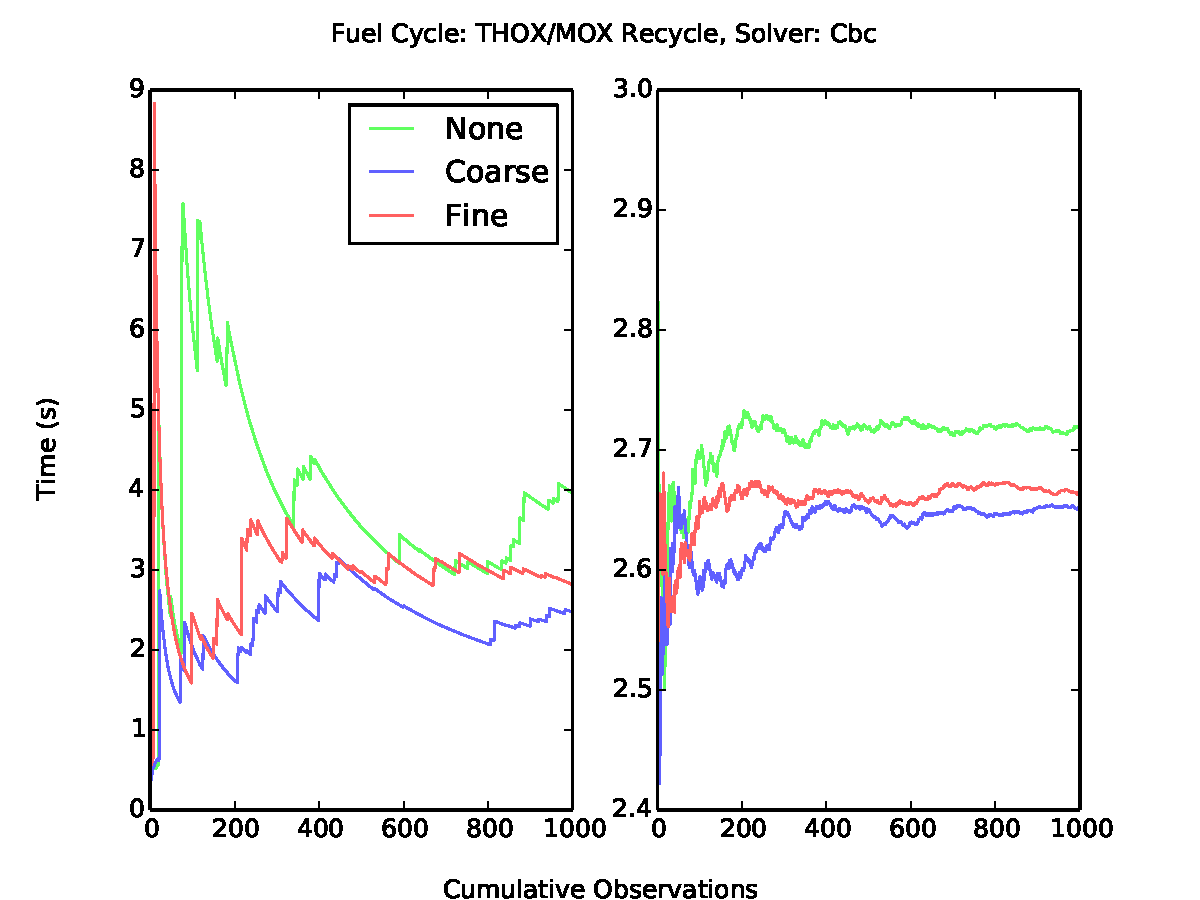
\includegraphics[width=.7\textwidth]{1k_avg_front_time_fc2_cbc.pdf}
    \caption{
      \label{fig:1k_avg_front_time_fc2_cbc}
      Cumulative average solution time of the \cbc solver for the front-end ThOX
      fuel cycle.}
  \end{center}
\end{figure}

Given the variety in stability by fuel cycle, viewing the underlying timing
distributions can also provide insight. Accordingly, Figure
\ref{fig:1k_hist_front_rx0} shows all timing distributions for low-fidelity
reactor models, and Figure \ref{fig:1k_hist_front_rx1} displays the
corresponding results for high-fidelity models.

\begin{figure}[h!]
  \begin{center}
    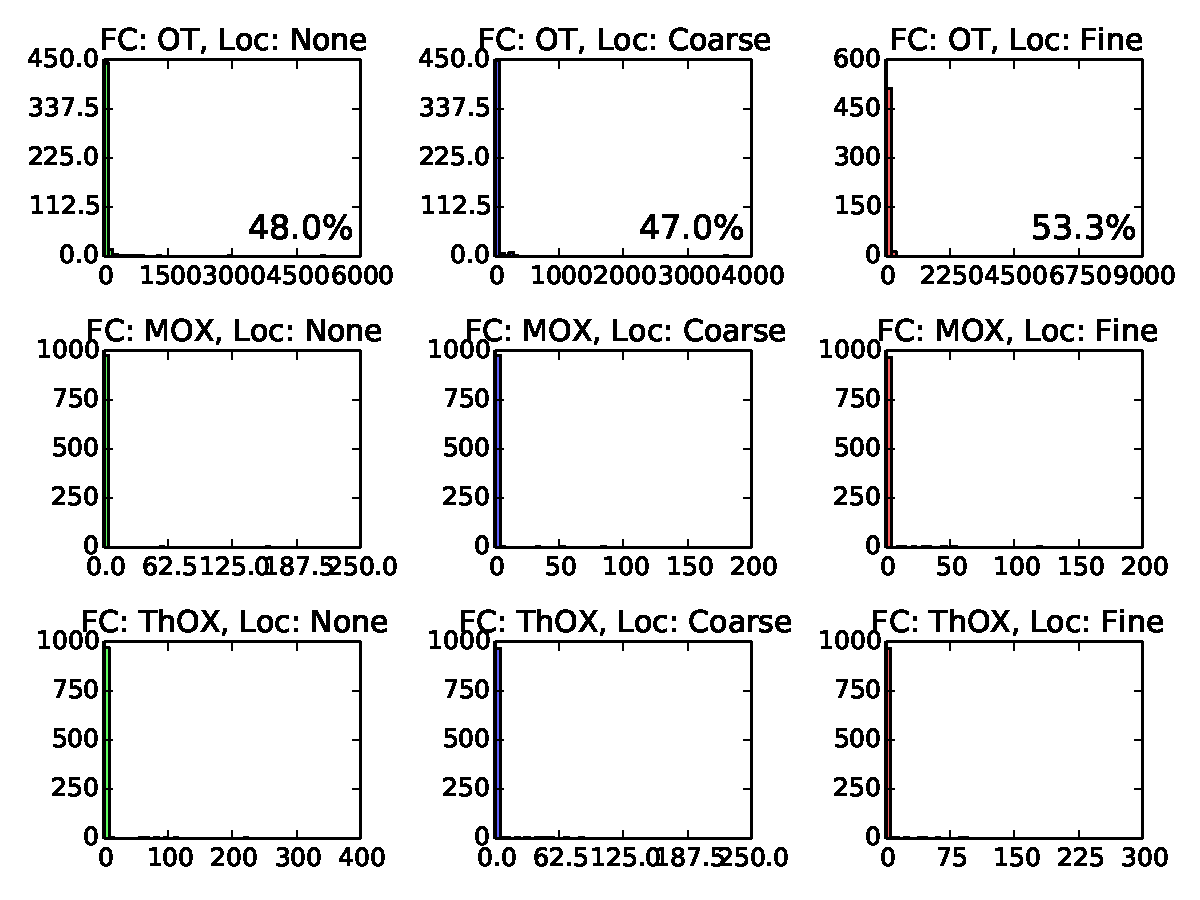
\includegraphics[width=.7\textwidth]{1k_hist_front_rx0.pdf}
    \caption{
      \label{fig:1k_hist_front_rx0}
      The distribution of converged solution times for all low-fidelity reactor
      instances. Outliers have been filtered out in order to show distribution
      shape. Fuel cycle fidelity increases from top to bottom, and location
      fidelity increases from right to left. The percentage of instance
      population shown is provided in black, if relevant. The percentages of all
      converged instances is shown in red, if relevant.}
  \end{center}
\end{figure}

\begin{figure}[h!]
  \begin{center}
    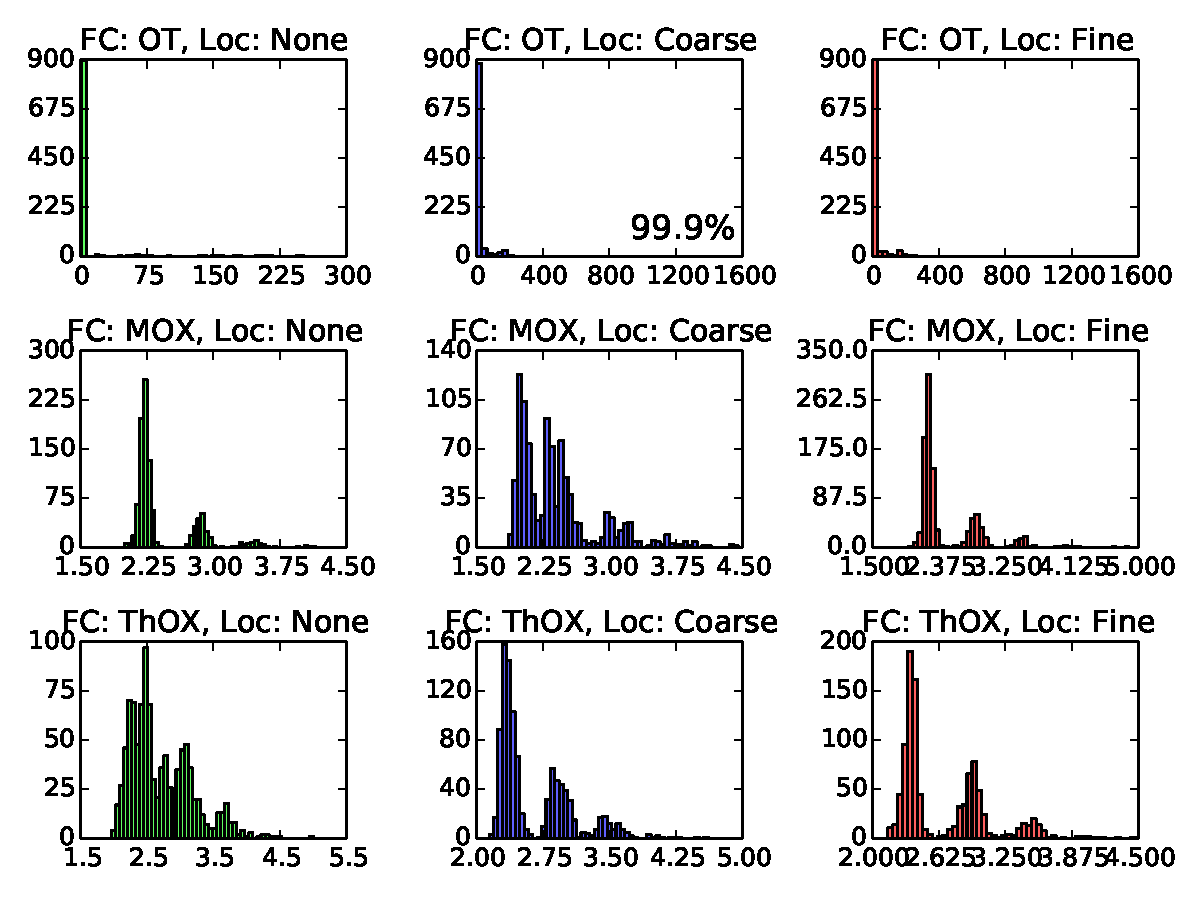
\includegraphics[width=.7\textwidth]{1k_hist_front_rx1.pdf}
    \caption{
      \label{fig:1k_hist_front_rx1}
      The distribution of converged solution times for all high-fidelity reactor
      instances. Fuel cycle fidelity increases from top to bottom, and location
      fidelity increases from right to left. Percentages are identical to Figure
      \ref{fig:1k_hist_front_rx0}.}
  \end{center}
\end{figure}

A number of interesting features exist in the figures related to the \cbc timing
study. Significantly, reactors in batch-mode have poor convergence for
once-through cycles, regardless of location parameter. This echoes observations
in the scaling study. For the remaining fuel cycles, outliers consistently are
observed for low-fidelity reactor models, also regardless of location
parameter. This effect is seen in the cumulative observation figures most
easily. Each occurrence of a timing outlier causes a large jump in the
observation. The converged, non-outlier instances with location-based
preferences show single-mode structure, whereas those without location
preferences appear to be bi-modal.

Conversely, high-fidelity reactor instances were found to almost always
converge. Outliers were found in the once-through fuel cycle results, but not in
other fuel cycles. Again, this behavior results in choppy cumulative
observations. Both the MOX and ThOX fuel cycles were shown to be comparatively
stable. Further, both cases have clear tri-modal solution-time populations.

\subsubsection{Simulation Objective vs. Solution Time}

The trade off of choosing to use a full-fledged optimization solver over a
heuristic is one between solution fidelity and solution time. Figure
\ref{fig:1k_compare_front_pref_flow} shows a comparison between the \cbc and
Greedy solvers. For each instance, relative simulation-objective values were
computed as shown in Equation \ref{eqn:sim_flow_compare}. Similarly, relative
solution times were computed. The average result found for high-fidelity reactor
instances solved with \cbc was taken as a reference point, plotted at the origin
in Figure \ref{fig:1k_compare_front_pref_flow}. Values are plotted for each
combination of fundamental parameters. A data point's position along the x-axis
indicates the average deviation from the high-fidelity model's simulation
objective, i.e., the dot product of preference and system flow. The y-axis
position indicates the average relative time difference.

\begin{figure}[h!]
  \begin{center}
    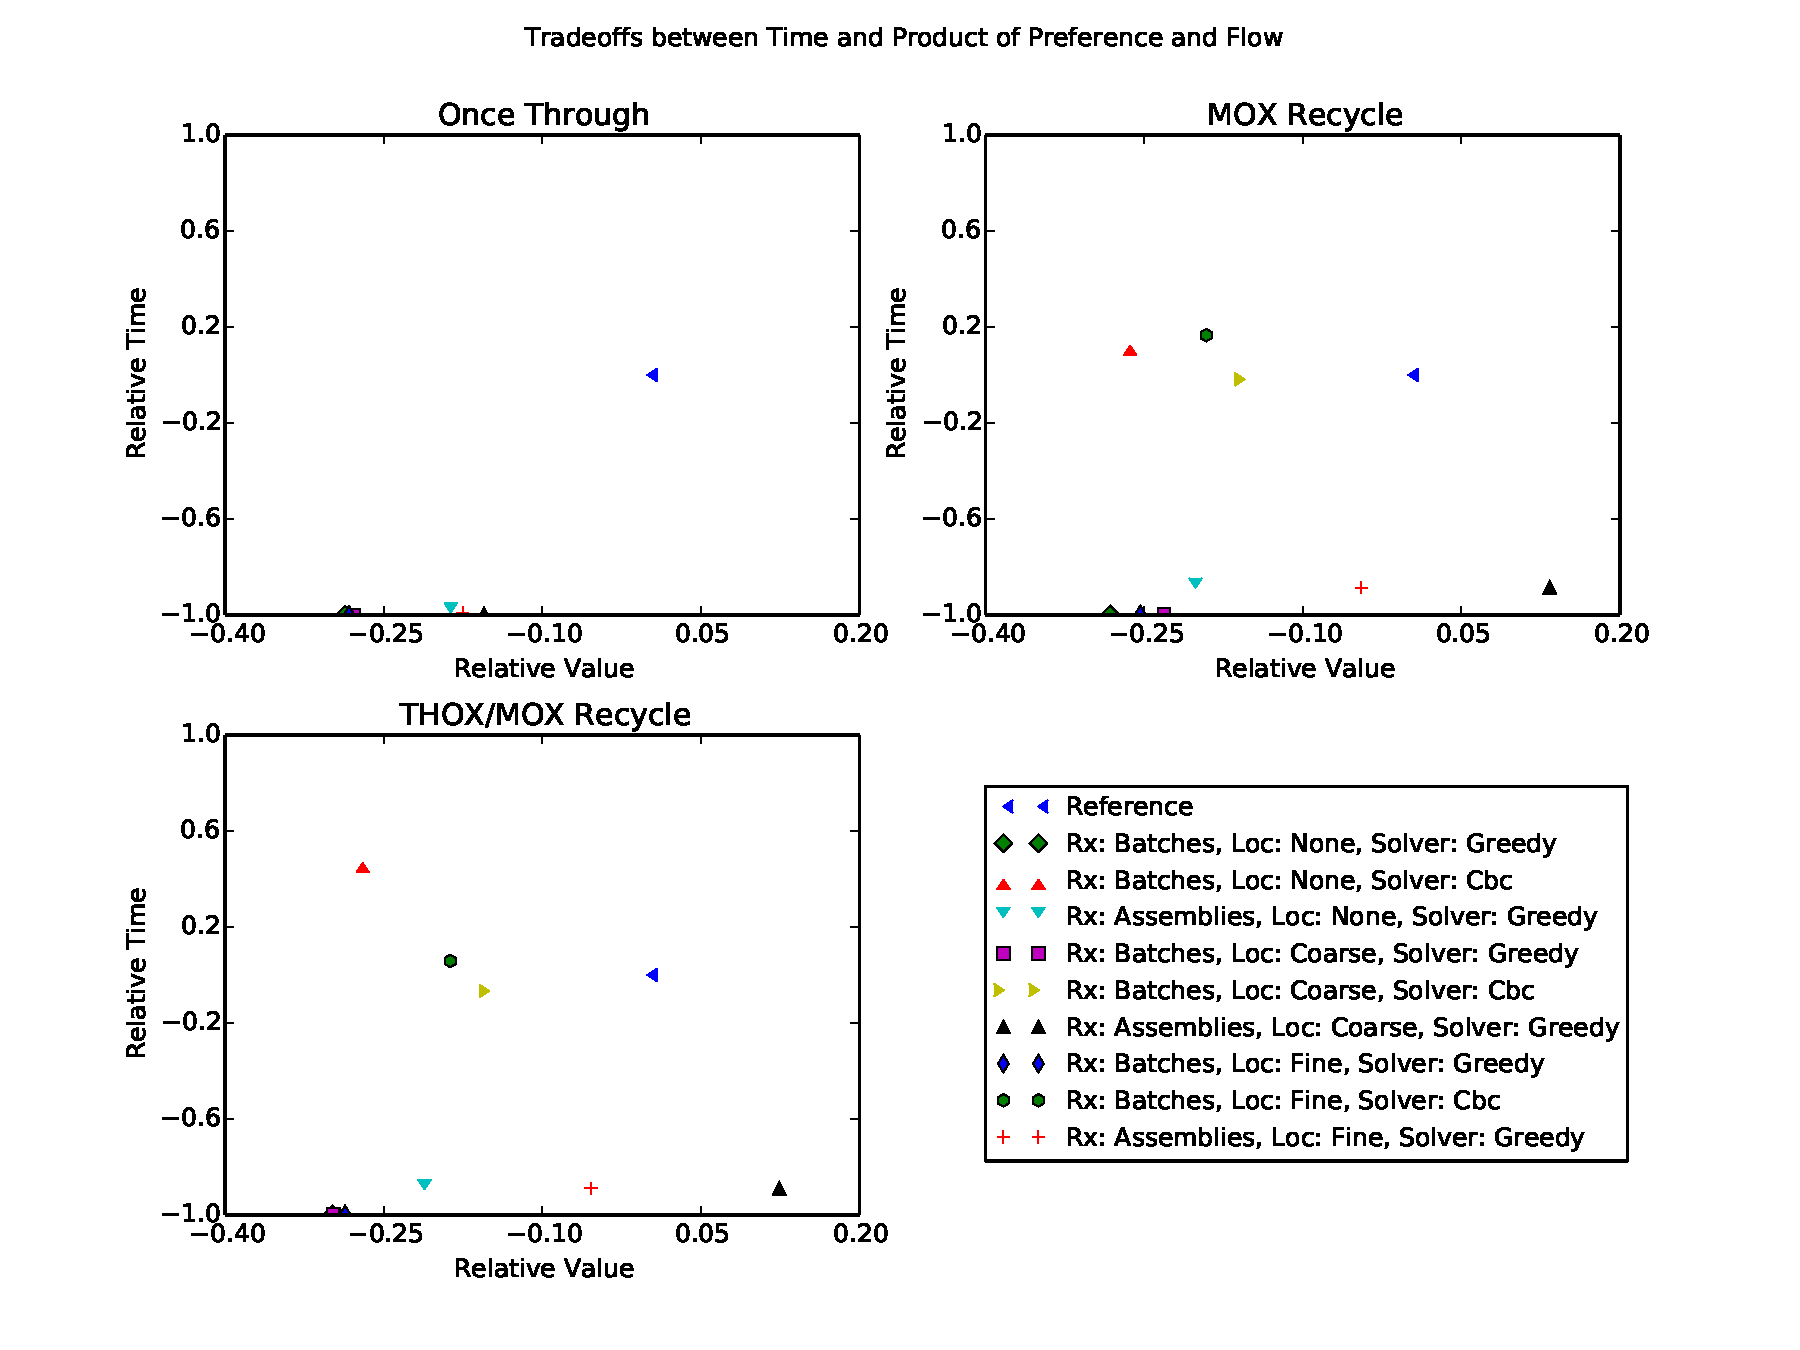
\includegraphics[width=.7\textwidth]{1k_compare_front_pref_flow.pdf}
    \caption{
      \label{fig:1k_compare_front_pref_flow}
      A comparison of simulation-objective values and solution times between
      instances solved with Greedy and \cbc solvers. Reference values are
      comprised of high-fidelity reactor instances solved with \cbc. Each other
      combination of fundamental parameter and solvers are then compared agaisnt
      the reference. Note that the once-through fuel cycle pane does not include
      other \cbc solvers, because their solution times were very long.
    }
  \end{center}
\end{figure}

In most every case, the results are as expected. The high-fidelity, \cbc-based
solution provides a better simulation objective for a more expensive time. In
general, the Greedy always performs much faster than \cbc, as expected from a
heuristic. Except for the Once-through case, all \cbc solves require similar
times, and the highest fidelity simulation provides the answer with the highest
objective measure. However, as was seen in the scalability study, the \cbc does
not always provide a better simulation-based metric when large costs are
concerned. Interestingly, the coarse-location fidelity Greedy solver results
provided a better average simulation objective.

\subsubsection{False Arc Cost Effects}

As was shown for previously, providing a small pseudo cost results in a higher
simulation-based objective metric. For example, Figure
\ref{fig:1k_compare_front_pref_flow} displayed results in which the Greedy
solver provided a higher average simulation-based metric than the \cbc
solver. Figure \ref{fig:cost_avg_front_pref_flow_fc1_} displays the underlying
data with additional data for small-cost \cbc solves. As can be seen, in the
lower center pane, the average preference-flow metric increases in a
\cbc-high-cost, Greedy, \cbc-low-cost order.

\begin{figure}[h!]
  \begin{center}
    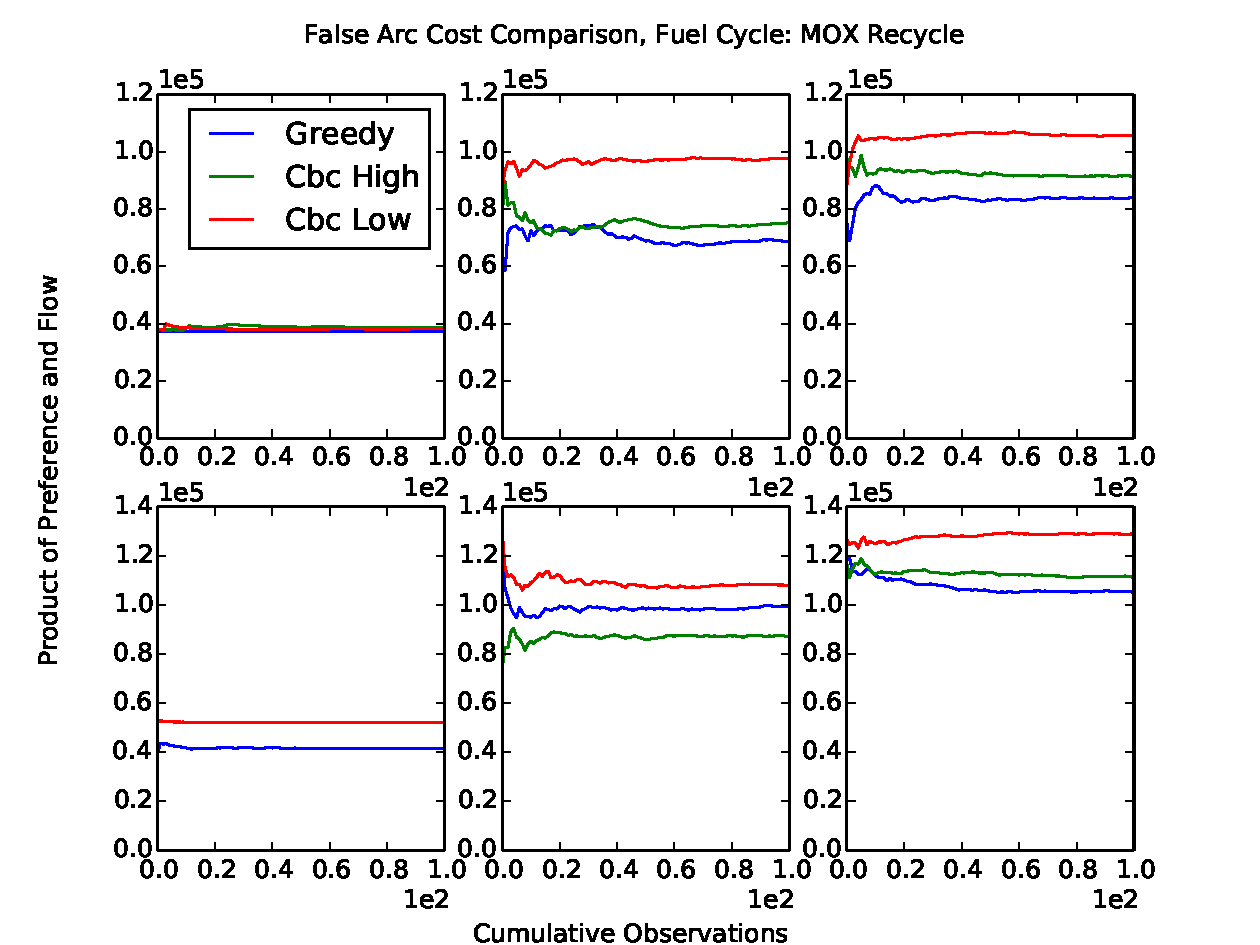
\includegraphics[width=.7\textwidth]{cost_avg_front_pref_flow_fc1_.pdf}
    \caption{
      \label{fig:cost_avg_front_pref_flow_fc1_}
      Simulation-objective values for 100 instances solved with the Greedy
      solver, a \cbc solver with a high false arc cost, and the \cbc solver with a
      low false arc cost.}
  \end{center}
\end{figure}

%% \subsubsection{Preference Conditioning Effects}

%% The relative weight provided to location over commodity preference does not
%% affect solution time.

%% \begin{figure}[h!]
%%   \begin{center}
%%     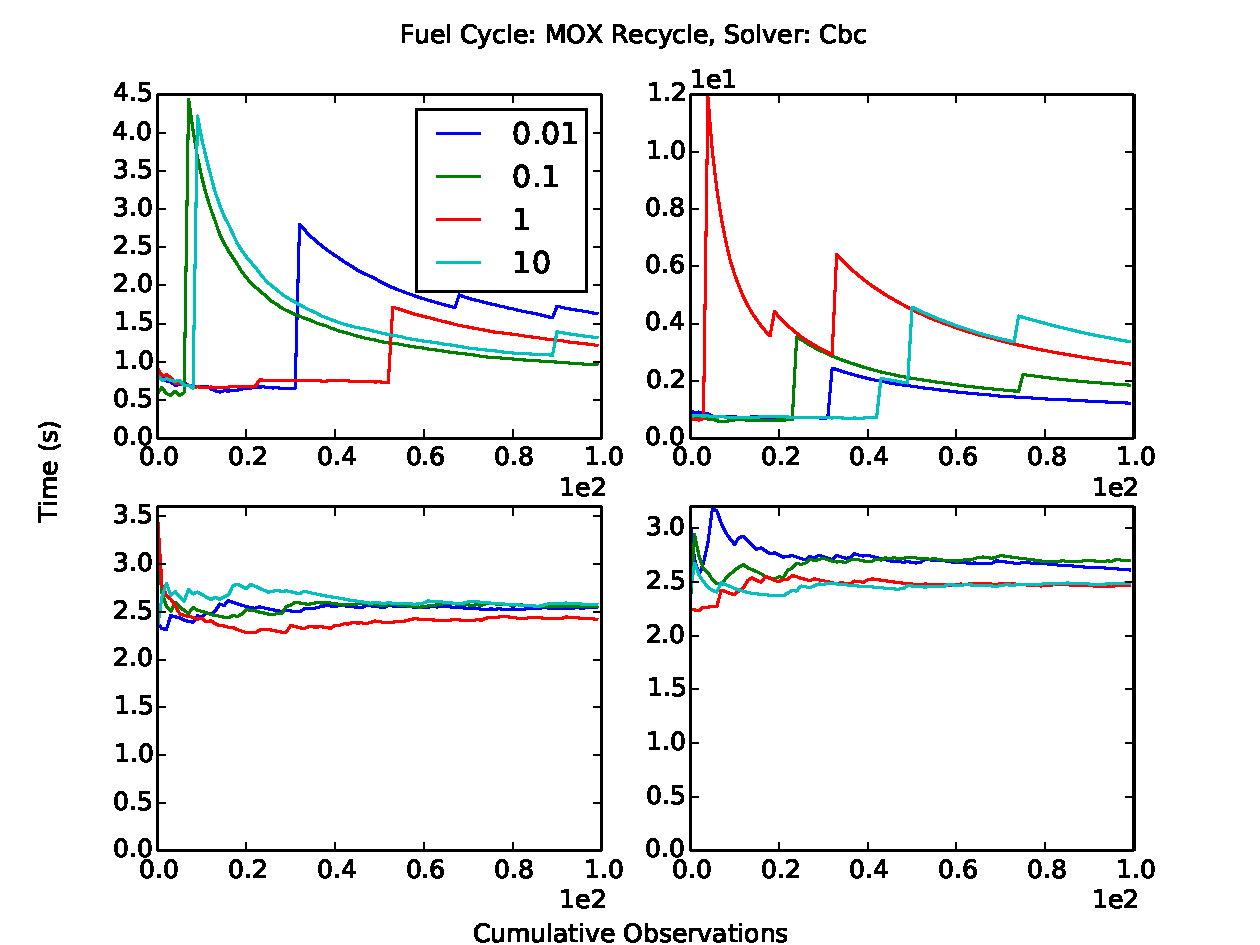
\includegraphics[width=.7\textwidth]{rlc_avg_front_time_fc1_cbc.pdf}
%%     \caption{
%%       \label{fig:rlc_avg_front_time_fc1_cbc}
%%       Caption.}
%%   \end{center}
%% \end{figure}

\subsection{Back-End Exchanges}

As with the scalability study, back-end exchanges perform quite similarly to
front-end exchanges. Accordingly, basic results are reviewed, and results that
lead to recommendations are discussed in more detail.

%% \subsubsection{Fundamental Parameter Variation}

Both the Greedy and \clp solvers again proved to have relatively stable solution
times. An example of the Greedy solver observed solution times for the MOX fuel
cycle is shown in Figure \ref{fig:1k_avg_back_time_fc1_greedy}. \clp results are
shown in Figure \ref{fig:1k_avg_back_time_fc1_clp}. 

\begin{figure}[h!]
  \begin{center}
    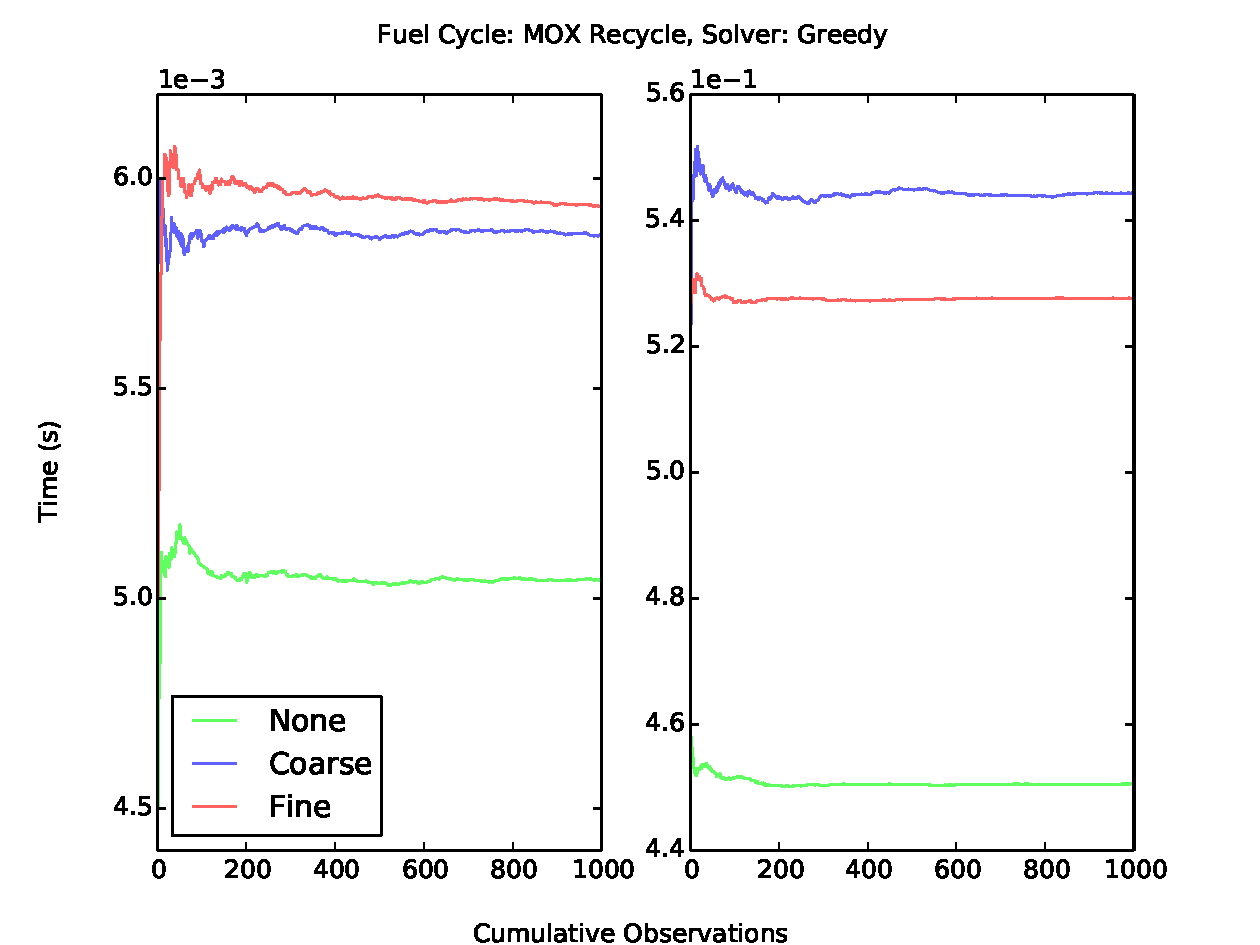
\includegraphics[width=.7\textwidth]{1k_avg_back_time_fc1_greedy.pdf}
    \caption{
      \label{fig:1k_avg_back_time_fc1_greedy}
      Cumulative average solution time of the Greedy solver for the back-end MOX
      fuel cycle.}
  \end{center}
\end{figure}

\begin{figure}[h!]
  \begin{center}
    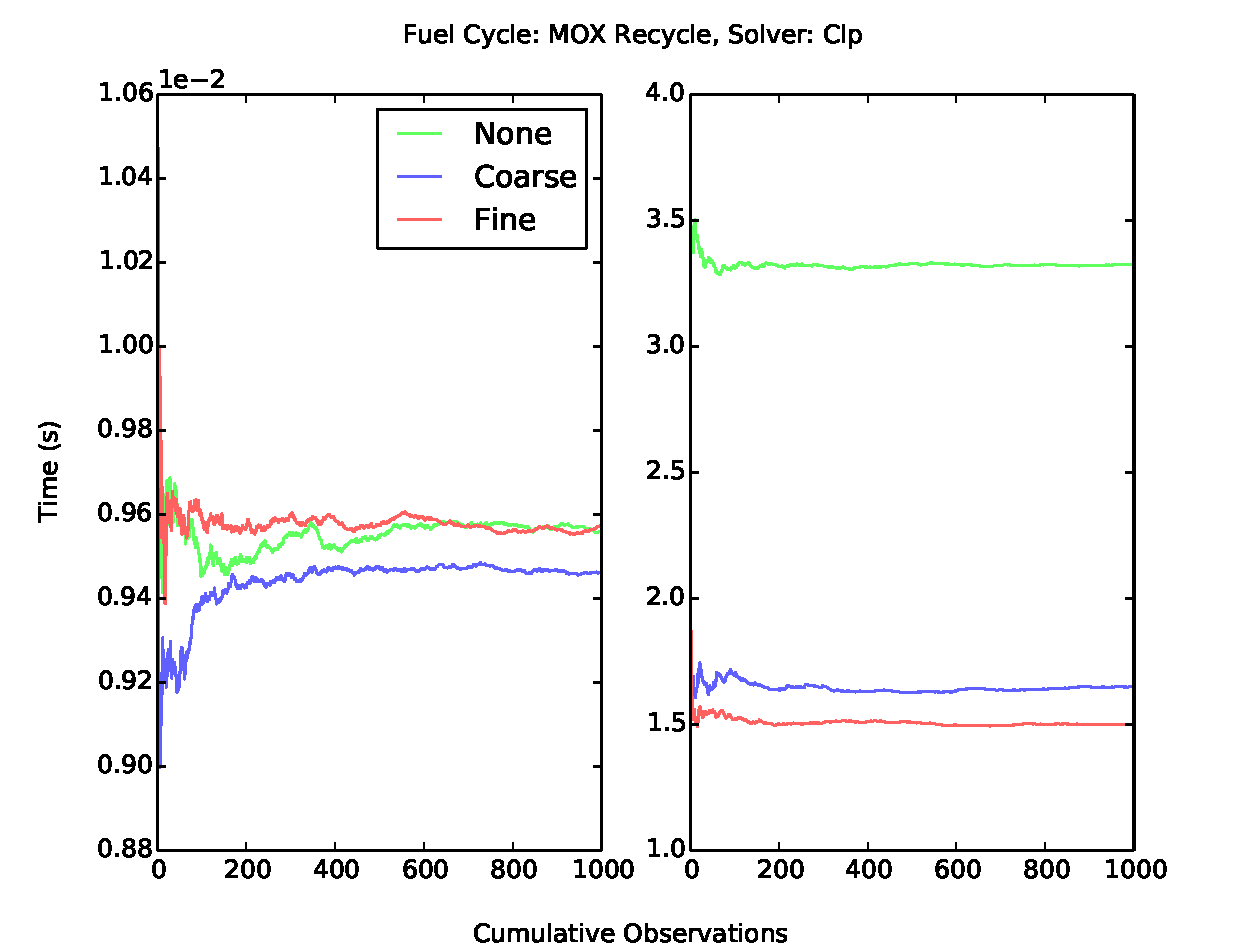
\includegraphics[width=.7\textwidth]{1k_avg_back_time_fc1_clp.pdf}
    \caption{
      \label{fig:1k_avg_back_time_fc1_clp}
      Cumulative average solution time of the \clp solver for the back-end MOX
      fuel cycle.}
  \end{center}
\end{figure}

The \clp solution time required for high-fidelity reactor models with no
location preference was found to be significantly higher than for instances
which included a location preference. A similar trend was found for \cbc
solutions, as shown in
\Cref{fig:1k_avg_back_time_fc1_cbc,fig:1k_avg_back_time_fc2_cbc} for the MOX and
ThOX fuel cycles, respectively. The timing discrepancy exists in low-fidelity
reactor models in the \cbc case, and is also much more pronounced. These results
indicate that solution times, in certain instances, can be significantly reduced
if solvers can better differentiate between arcs based on objective
coefficients. Therefore, a possible speed-up strategy can include ``salting''
the preference vector by adding a random $\delta_p$ to each entry. Such a
strategy will likely be useful in only certain cases, and should be tested only
if long run times are encountered.

\begin{figure}[h!]
  \begin{center}
    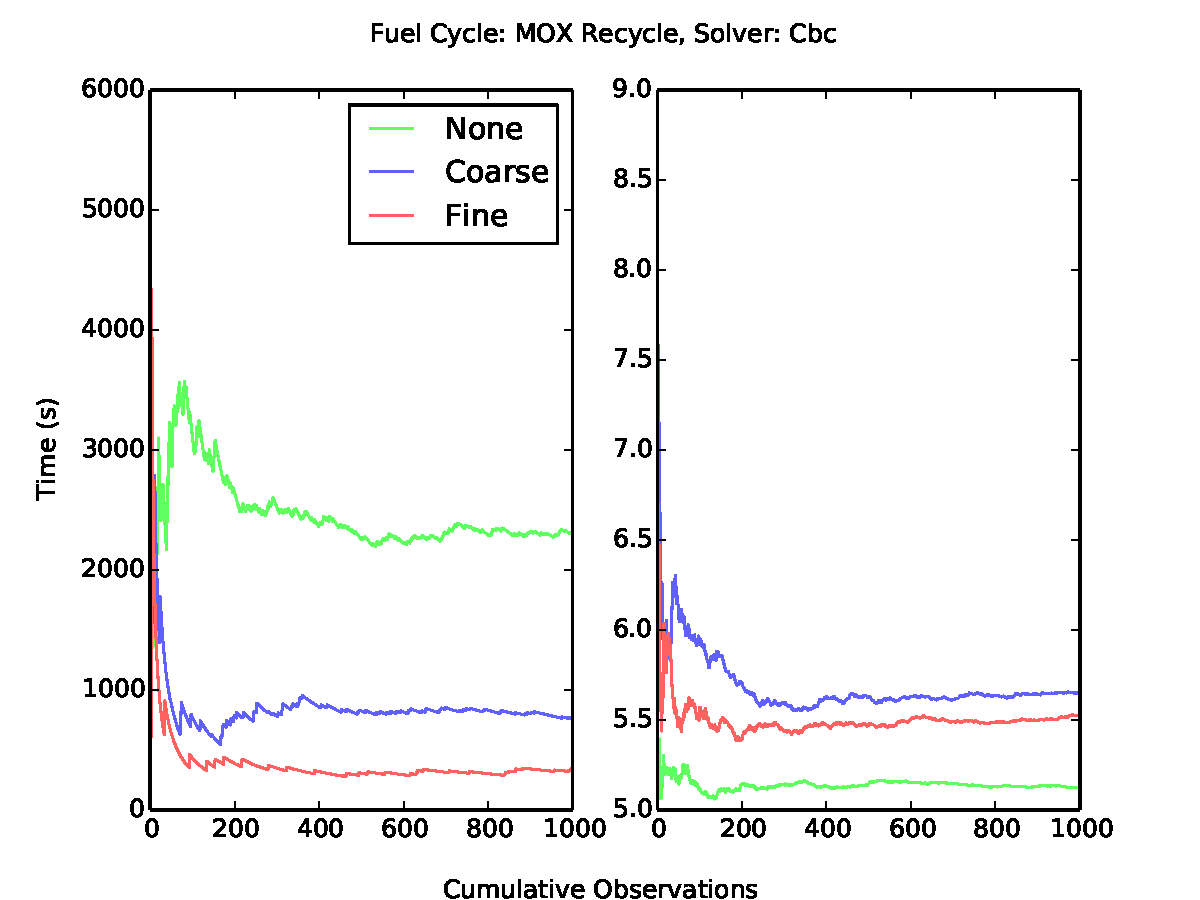
\includegraphics[width=.7\textwidth]{1k_avg_back_time_fc1_cbc.pdf}
    \caption{
      \label{fig:1k_avg_back_time_fc1_cbc}
      Cumulative average solution time of the \cbc solver for the back-end MOX
      fuel cycle.}
  \end{center}
\end{figure}

\begin{figure}[h!]
  \begin{center}
    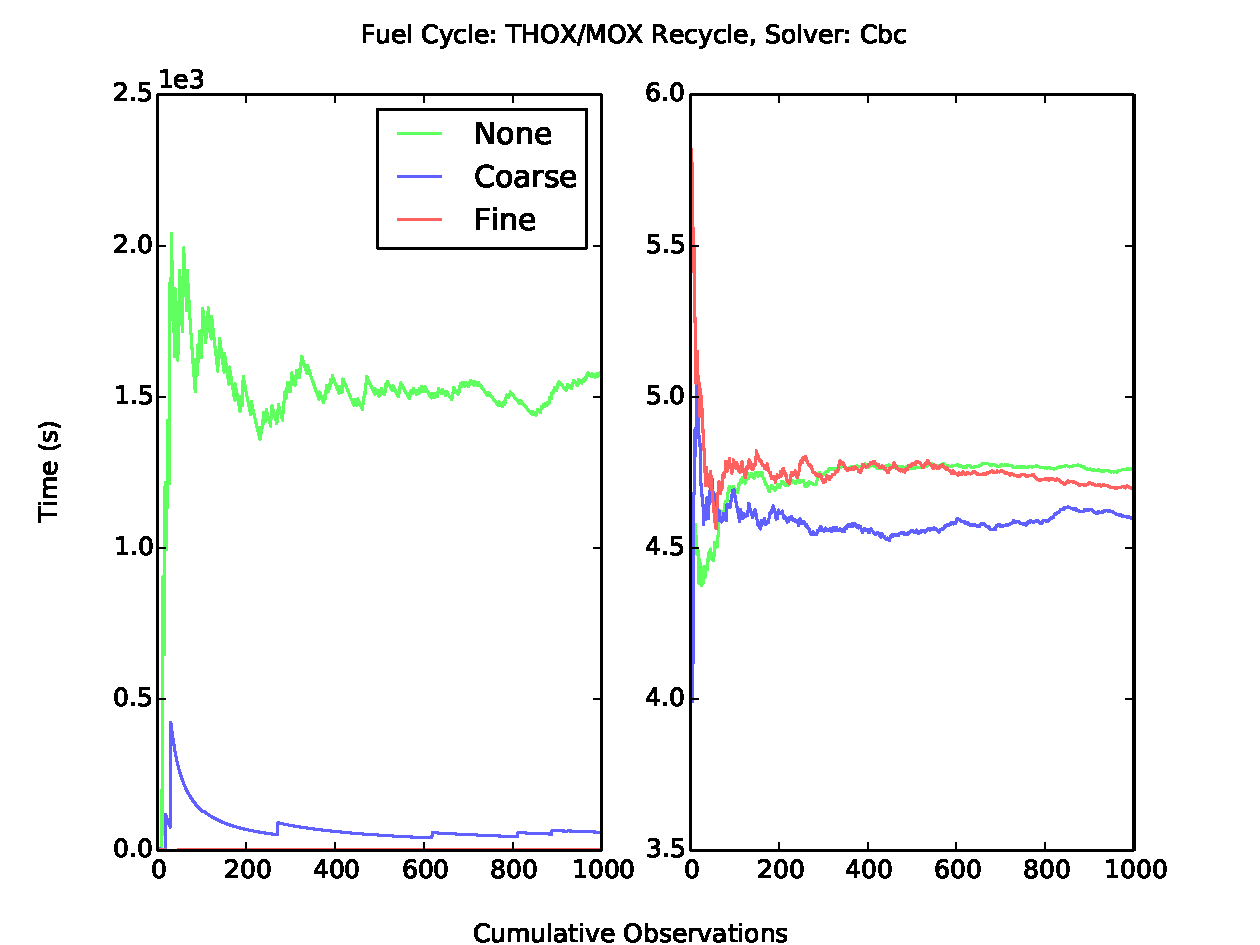
\includegraphics[width=.7\textwidth]{1k_avg_back_time_fc2_cbc.pdf}
    \caption{
      \label{fig:1k_avg_back_time_fc2_cbc}
      Cumulative average solution time of the \cbc solver for the back-end ThOX
      fuel cycle.}
  \end{center}
\end{figure}

%% \begin{figure}[h!]
%%   \begin{center}
%%     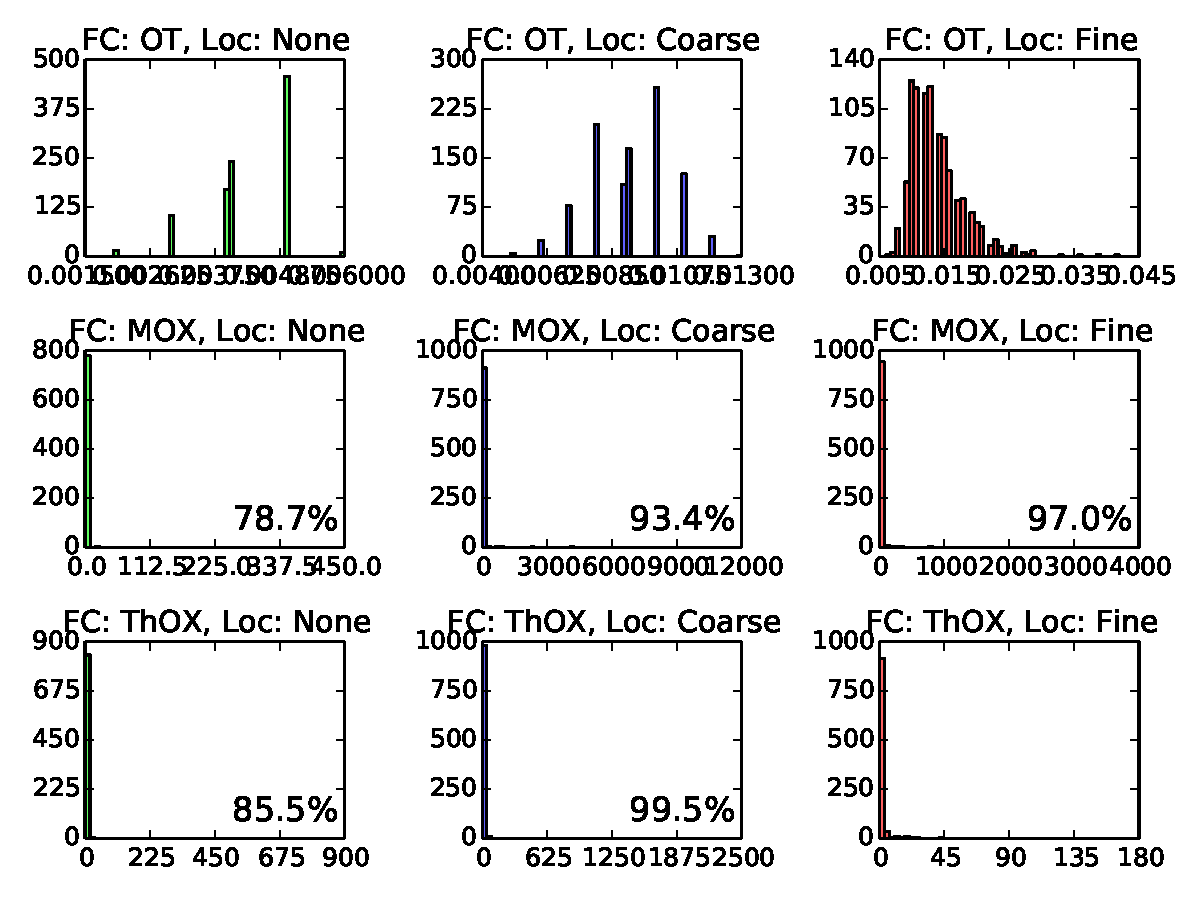
\includegraphics[width=.7\textwidth]{1k_hist_back_rx0.pdf}
%%     \caption{
%%       \label{fig:1k_hist_back_rx0}
%%       Caption.}
%%   \end{center}
%% \end{figure}

%% \begin{figure}[h!]
%%   \begin{center}
%%     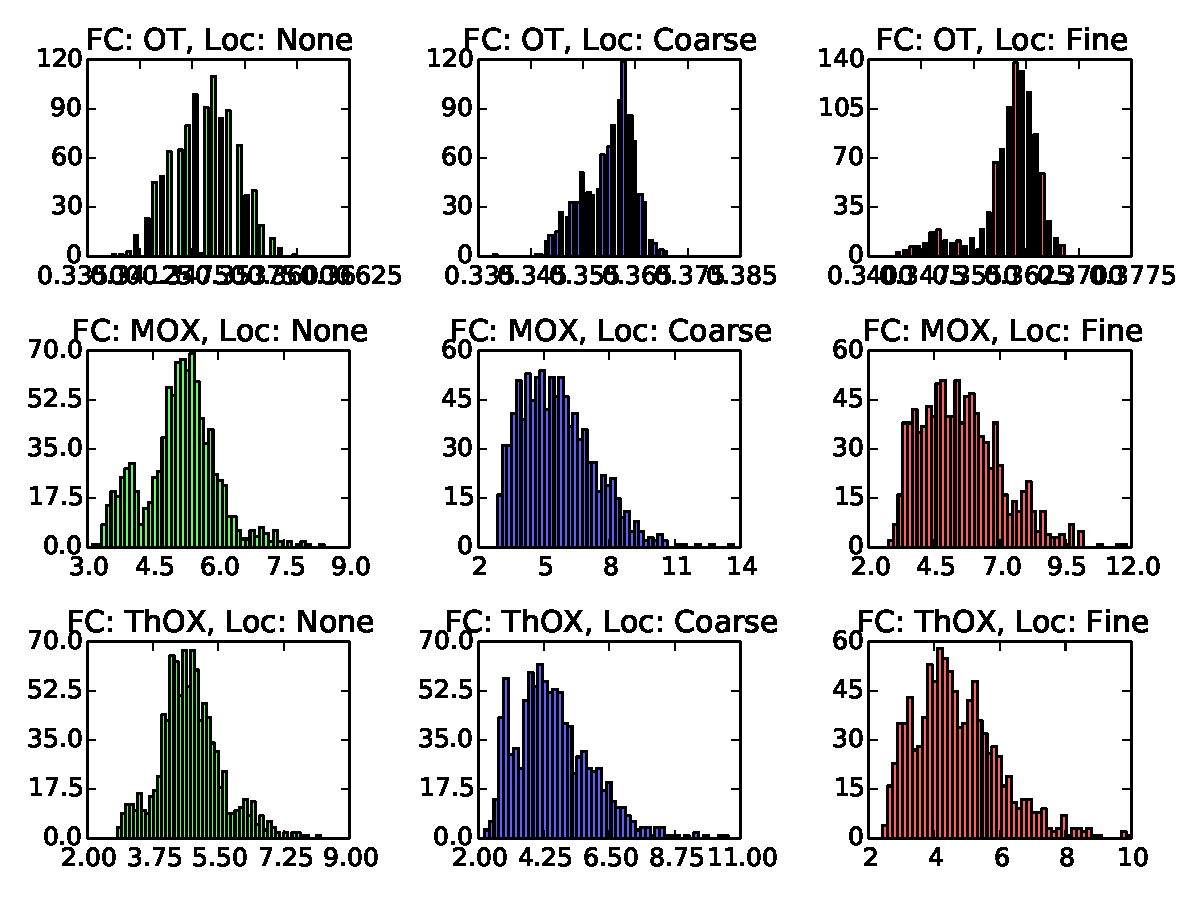
\includegraphics[width=.7\textwidth]{1k_hist_back_rx1.pdf}
%%     \caption{
%%       \label{fig:1k_hist_back_rx1}
%%       Caption.}
%%   \end{center}
%% \end{figure}

%% In the back-end case, lower-fidelity reactor models provide better
%% simulation-based metrics when using the \cbc solver. The higher-fidelity models
%% still maintain a better objective in cost space. This behavior is not reversed
%% for all fuel cycles when moving to a lower artificial-arc cost, suggesting that
%% the model is sensitive to the preference-to-cost translation function.

%% \begin{figure}[h!]
%%   \begin{center}
%%     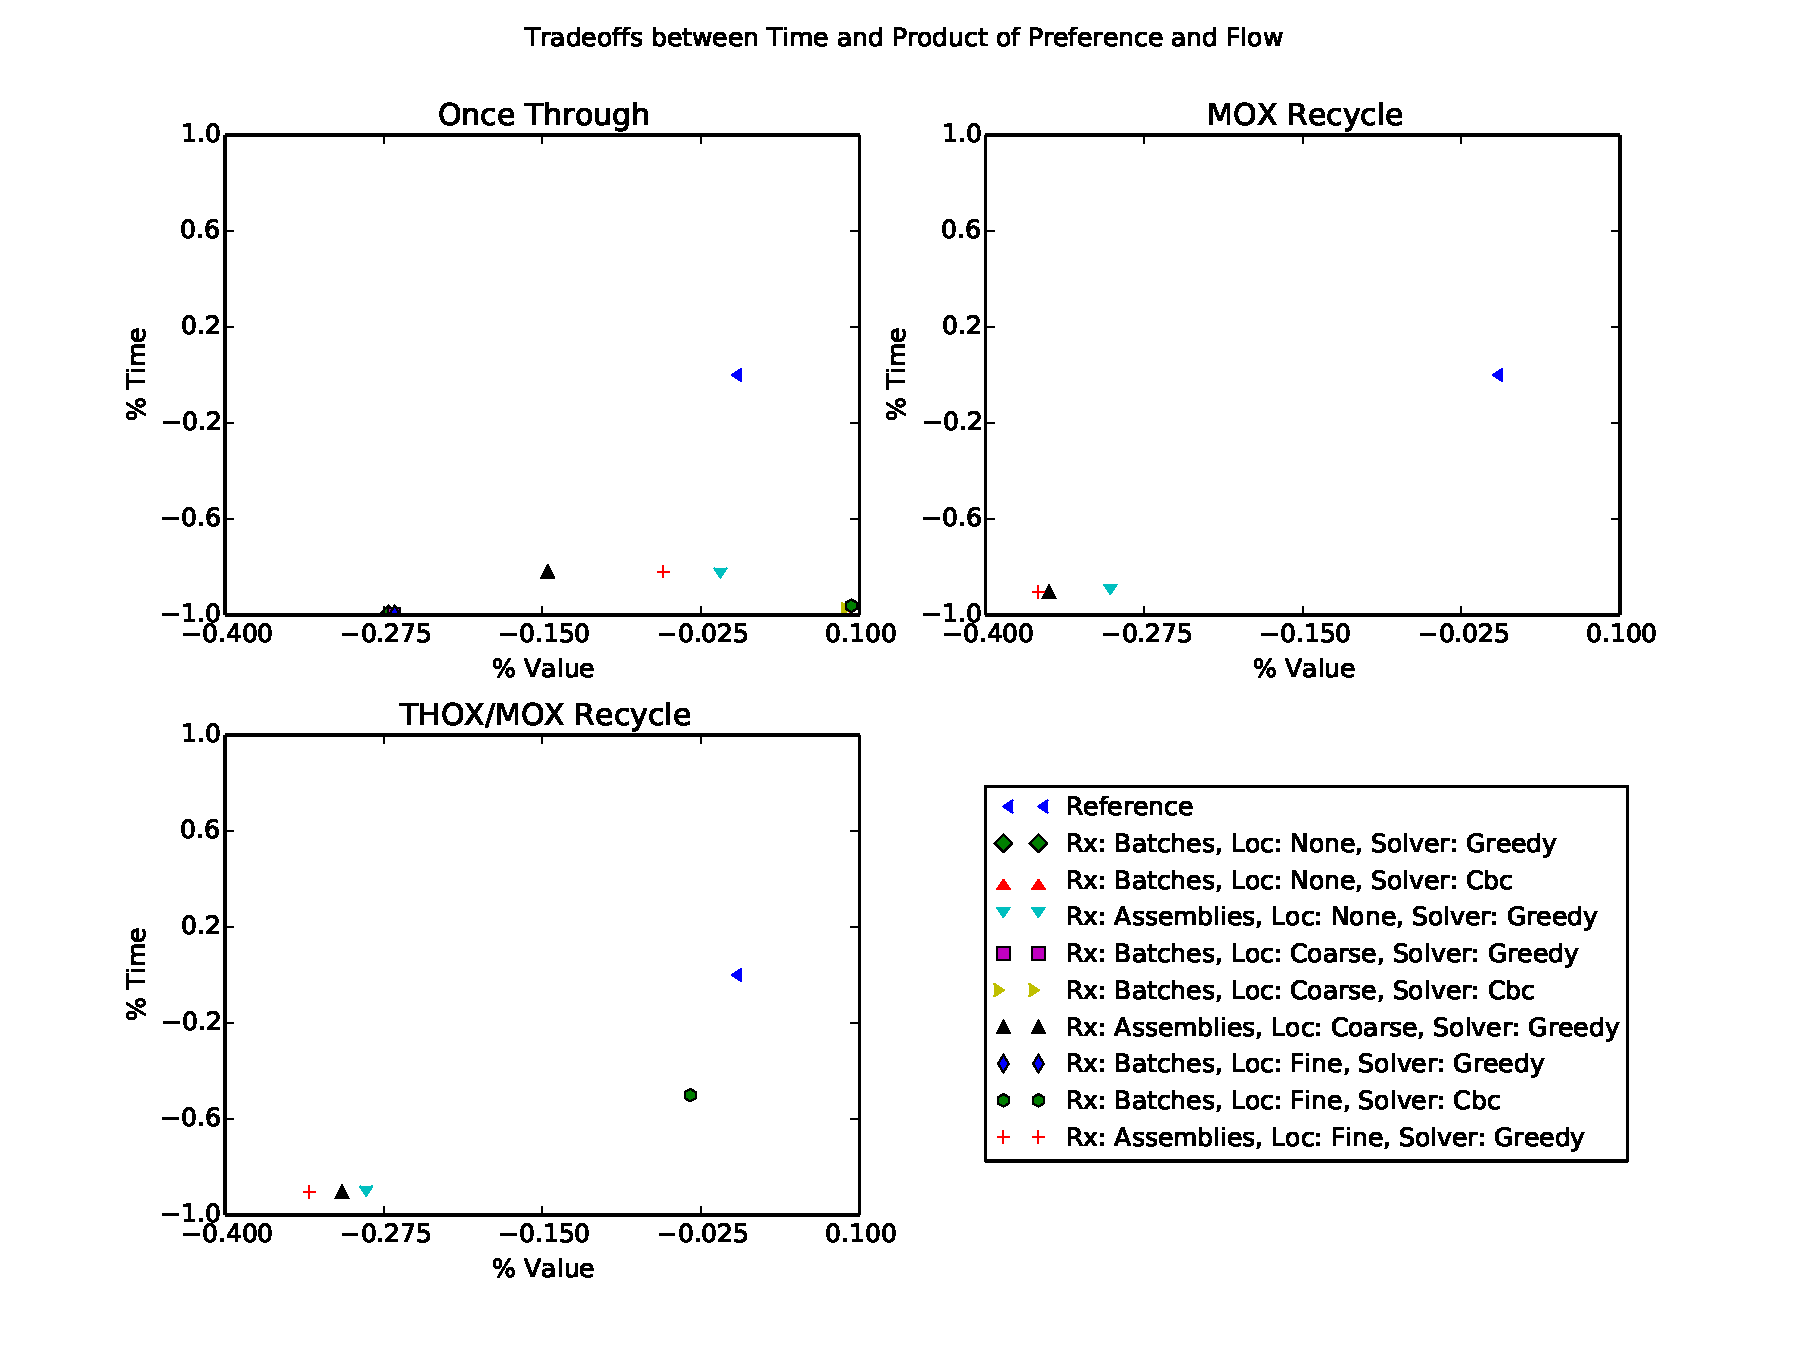
\includegraphics[width=.7\textwidth]{1k_compare_back_pref_flow.pdf}
%%     \caption{
%%       \label{fig:1k_compare_back_pref_flow}
%%       Caption.}
%%   \end{center}
%% \end{figure}

%% \subsubsection{Preference Conditioning Effects}

%% In some cases, having a small or large location-based preference showed
%% significant performance effects. 

%% \begin{figure}[h!]
%%   \begin{center}
%%     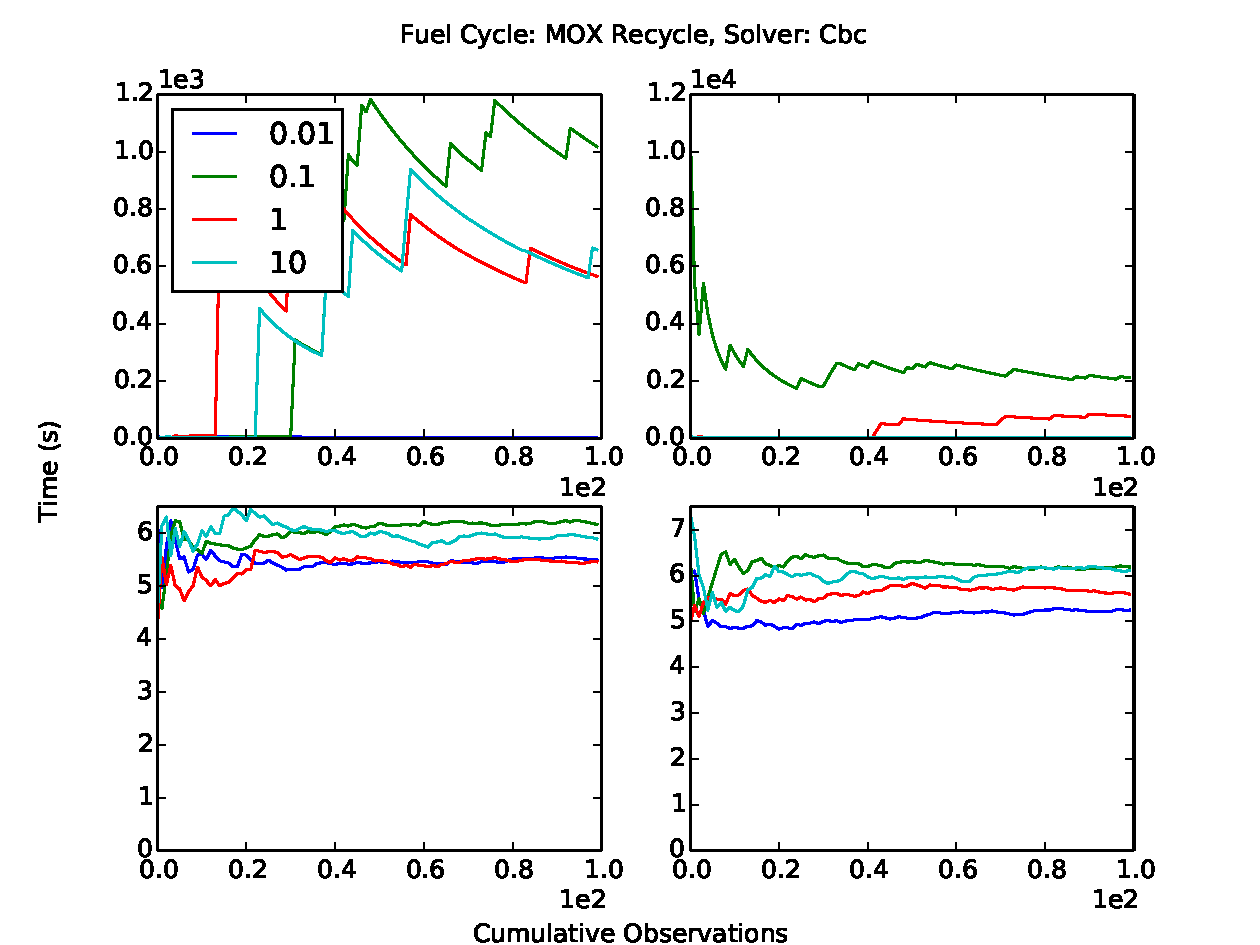
\includegraphics[width=.7\textwidth]{rlc_avg_back_time_fc1_cbc.pdf}
%%     \caption{
%%       \label{fig:rlc_avg_back_time_fc1_cbc}
%%       Caption.}
%%   \end{center}
%% \end{figure}

%% With a small location preference value, preference flows are effectively unaltered.

%% \begin{figure}[h!]
%%   \begin{center}
%%     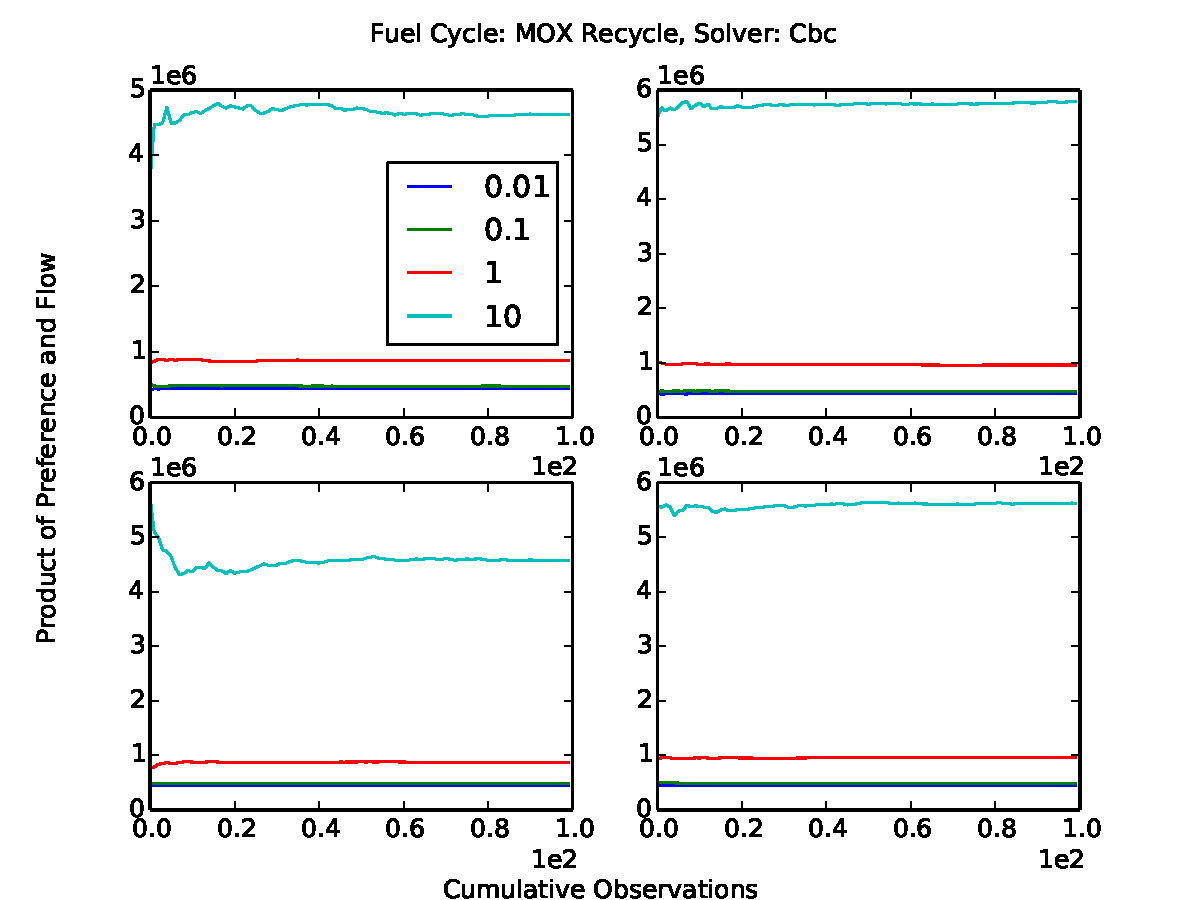
\includegraphics[width=.7\textwidth]{rlc_avg_back_pref_flow_fc1_cbc.pdf}
%%     \caption{
%%       \label{fig:rlc_avg_back_pref_flow_fc1_cbc}
%%       Caption.}
%%   \end{center}
%% \end{figure}

